\section{Introduction}
\label{sec:introduction}

\subsection{Problem statement}
\label{sec:prob_stmt}

\begin{figure}
  \centering
  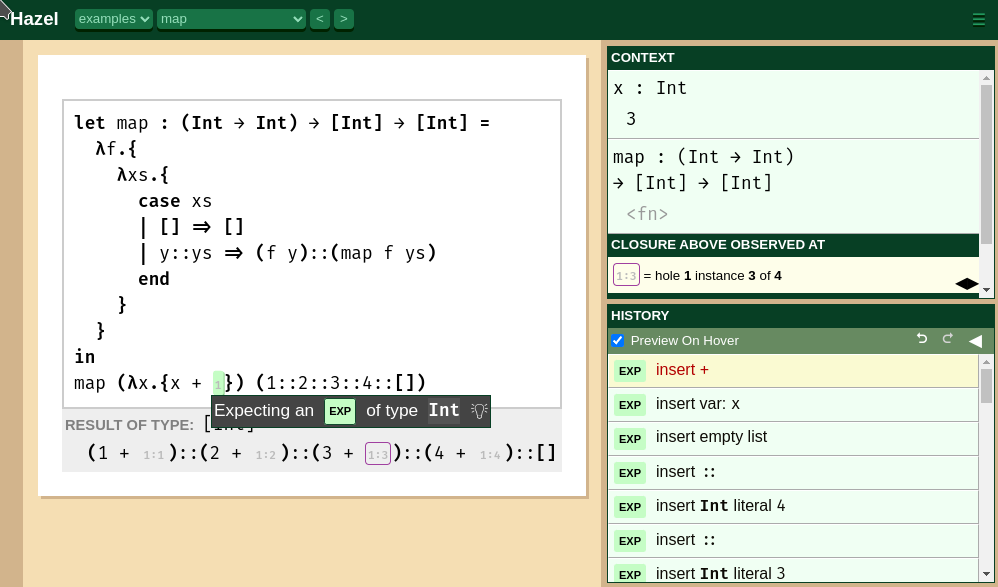
\includegraphics[width=4in]{img/hazel_ui.png}
  \caption[Screenshot of the Hazel live programming environment.]{A screenshot of the Hazel live programming environment. Screenshot taken of the dev branch demo\footnotemark{} on 02/06/2022.}
  \label{fig:screenshot-hazel-ui}
\end{figure}

% https://tex.stackexchange.com/a/10185
\footnotetext{\url{https://hazel.org/build/dev/}}

\subsection{The contribution of this work}
\label{sec:contribution}

\subsection{Structural overview}
\label{sec:structural_overview}

\Cref{sec:background} provides a background on necessary topics in programming language (PL) theory and programming language implementations, in order to frame understanding for the Hazel live programming environment. \Cref{sec:hazel} provides an overview of Hazel, in order to frame the work completed for this thesis project. \Crefrange{sec:env_model_evaluation}{sec:far_impl} describe the primary work completed for this project, as described in \Cref{sec:contribution}. \Cref{sec:far_eval} comprises an assessment of the work completed in terms of correctness and the theoretical performance. \Cref{sec:future_work} is a discussion of future research directions that may be spawned off from this work. \Cref{sec:concl} concludes with a summary of findings and future work. The appendices contain additional information about the Hazel project not directly related to the primary contribution of this project, as well as selected source code snippets.

%%% Local Variables:
%%% mode: latex
%%% TeX-master: "main"
%%% End:
